\documentclass{article}
\usepackage{amsmath}
\usepackage{graphicx}
\title{Sample Paper Title}
\author{Author Name}
\date{\today}

\begin{document}

\maketitle

\begin{abstract}
This is a sample abstract for the paper. It provides a brief overview of the content and findings of the research.
\end{abstract}

\section{Introduction}
The introduction section provides background information and outlines the objectives of the research.

\section{Methodology}
This section describes the methods used in the research, including any experimental setups or data collection techniques.

\section{Results}
Here, the results of the research are presented, including any relevant figures or tables.

\begin{figure}[h]
    \centering
    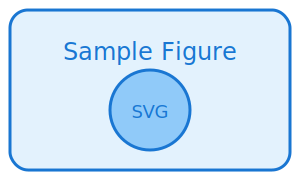
\includegraphics[width=0.5\textwidth]{../static/img/sample-figure.svg}
    \caption{Sample figure caption.}
    \label{fig:sample}
\end{figure}

\section{Discussion}
The discussion section interprets the results and discusses their implications in the context of existing research.

\section{Conclusion}
This section summarizes the main findings of the paper and suggests directions for future research.

\section*{References}
References should be formatted according to the chosen citation style.

\end{document}